\documentclass[xcolor=dvipsnames]{beamer}

\usepackage{pdfcomment}
\usepackage{xcolor}
\usepackage[ngerman]{babel} % deutsche Silbentrennung
\usepackage[utf8]{inputenc} % wegen deutschen Umlauten
\usepackage{pdfpages}
\usepackage{graphicx}
\usepackage{pst-node}% http://ctan.org/pkg/pst-node
\usepackage{eurosym}


\usetheme{metropolis}           % Use metropolis theme
\title{The smallest grammar problem}
\date{05. Juli 2019}
\author{Edgar Dorausch}
%\institute{Centre for Modern Beamer Themes}
\begin{document}
\maketitle


\newcommand{\SubItem}[1]{
  \setlength\itemindent{15pt} \item[-] #1
}
\newcommand{\Gap}{$ $ \linebreak}
\newcommand{\FrameName}{
	\ifthenelse{\equal{\subsecname}{}}{
		\secname
	}{
		\secname \thinspace -\thinspace\subsecname
	}
}

\newcommand{\Fresh}{\ddagger}
\newcommand{\Hint}[1]{\textcolor{gray}{#1}}

\newboolean{WithComments}
\setboolean{WithComments}{true}
\newcommand{\PDFC}[1]{
	\ifthenelse{\boolean{WithComments}}{
		\pdfcomment[color=red,icon=Note]{#1}
	}{
		% Empty
	}
}
% \newcommand{\PDFC}[1]{}

\section{Motivation und Anwendung}

\begin{frame}{\FrameName}
	\begin{itemize}[<+->]
		\item Kompression
		\item Mustererkennung \linebreak
		\Hint{z.B. DNA-Analyse, NLP}
	\end{itemize}
\end{frame}

\section{Definitionen und Wiederholung}
\begin{frame}{\FrameName}
	\begin{block}{Kontextfreie Grammatik}
		\Gap
		Eine KFG ist ein Quadrupel $(\Sigma,\Gamma,S,\Delta)$ mit
		\begin{itemize}
			%	\item \alert<4>{This is\only<4>{ really} important}
			\item $\Sigma$ - Terminalalphabet
			\item $\Gamma$ - Nichtterminalalphabet
			\item $S$ - Startsymbol
			\item $\Delta$ - Menge von Regeln der Form $T\rightarrow\alpha$\linebreak
			$T \in \Gamma$;
			$\alpha \in (\Sigma \cup \Gamma)^\ast$
		\end{itemize}
	\end{block}
	
\end{frame}

\begin{frame}{\FrameName}
\begin{alert}{Besonderheit:}
	\Gap
	Grammatiken sollen nur ein Wort erzeugen (straight-line grammar):
	\begin{itemize}
		
		\item Grammatik muss azyklisch sein
		\item Für jedes $T \in \Gamma$ existiert nur eine Regel in $\Delta$
	\end{itemize}
\end{alert}
\end{frame}

\begin{frame}{\FrameName}
\begin{block}{Expansion  eines Strings $\alpha$}
	\Gap
	Erschöpfendes Anwenden der Regeln \linebreak
	Notation: $\langle \alpha \rangle$

	\visible<2>{
		\Gap
		\textbf{Größe einer Grammatik G}
		\Gap
		Anzahl der Zeichen in den rechten Seiten der Grammatikregeln\linebreak
		Notation: $m = \lvert G \lvert = \sum\limits_{(T \rightarrow \alpha) \in \Delta} | \alpha |$ \linebreak $ $\linebreak
		Größe der kleinsten Grammatik für einen String: $m^*$}
\end{block}
\end{frame}

\begin{frame}{\FrameName}
\begin{block}{Beispiel}
	$$
	G \colon \begin{Bmatrix} 
		S \rightarrow rhaTber \textvisiblespace TTa \\
		T \rightarrow bar
	\end{Bmatrix}
	$$
	
	$\langle S \rangle = rhabarber \textvisiblespace barbara$ \linebreak
	$| \langle S \rangle| = 17$ \linebreak
	$\lvert G \lvert = 11$
\end{block}
\end{frame}

\begin{frame}{\FrameName}
\begin{block}{Approximation Ratio}
	\Gap
	Sei $G_A$ die Grammatik, die von einem Algorithmus $A$ erzeugt wird.
	$$
	a(n) = \alert<2>{\max\limits_{\alpha \in \Sigma^n}}\frac{
		\textrm{$\lvert G_A \lvert$ für $\alpha$}
	}{
		\textrm{$m^*$ für $\alpha$}
	}
	$$
	\begin{center}\alert{
			
			\visible<2>{Worstcase!}
		}
	\end{center}
	
\end{block}
\end{frame}

\begin{frame}{\FrameName}
\begin{table}
	\caption{Landau Notation}
	\begin{tabular}{ r p{3.5cm} l}
		
		$f \in o(g)$ & "$f < g$" \\
		%$\only<1>{f \in \mathcal{O}(g)}\only<2>{\alert{f \in \mathcal{O}(g)}}$ & "$f\leq g$" \\
		\textcolor{gray}{(Upper bound)} $f \in \mathcal{O}(g)$ & "$f\leq g$" \\
		$f \in \Theta(g)$ & "$f = g$"\\
		\textcolor{gray}{(Lower bound)} $f \in \Omega(g)$ & "$f \geq g$"\\
		$f \in \omega(g)$ & "$f > g$"\\
	\end{tabular}
\end{table}
\end{frame}

\section{Lemmata}

\begin{frame}{\FrameName}
\begin{block}{Lemma 1}
  \begin{center}
    \fbox{
      $
      m^* \in \Omega(log(n))
      $
    }
  \end{center}
  \begin{center}
    \Hint{(Ohne Beweis)}
  \end{center}
  
\end{block}
\end{frame}

\begin{frame}{\FrameName}
\begin{block}{Lemma 2a}
  \begin{center}
    \fbox{
      Es gibt Grammatik der Größe $|G_\alpha| + |G_\beta| + 2$ für $\alpha \beta$.
    }
  \end{center}
  \begin{itemize}
    \item<2-> $G_\alpha$ und $G_\beta$ vereinigen
    \item<3-> Neue Startregel: $S \rightarrow S_\alpha S_\beta$
  \end{itemize}
  
\end{block}
\end{frame}

\begin{frame}{\FrameName}
  \begin{block}{Lemma 2b}
    \begin{center}
      \fbox{
        Es gibt Grammatik der Größe $|G_\alpha| + \mathcal{O}(log(k))$ für $\alpha^k$.
      }
    \end{center}
    \begin{itemize}
      \item<2-> Neue Regeln baumartig strukturieren
      \item<3-> Baum hat nur logarithmische Höhe
    \end{itemize}
    \visible<4->{
      
      \begin{minipage}[h]{0.3\textwidth} 
        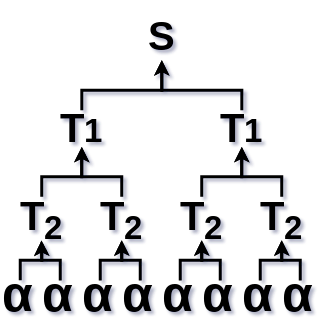
\includegraphics[width=\textwidth]{Images/Definitions/Tree.png}
     \end{minipage}
     \begin{minipage}[h]{0.5\textwidth}
      $$S \rightarrow T_1 T_1 $$
      $$T_1 \rightarrow T_2 T_2 $$
      $$T_2 \rightarrow \alpha \alpha $$
     \end{minipage}
    }

    
  \end{block}
    \end{frame}

\begin{frame}{\FrameName}
  \begin{block}{Lemma 3 \Hint{(mk-Lemma)}}
    \begin{center}
      \fbox{\begin{tabular}{@{}c@{}}
        In einem String gibt es maximal $mk$ \underline{unterschiedliche} \\ Substrings der Länge $k$
      \end{tabular}}
    \end{center}

    \begin{center}
      \Hint{(Ohne Beweis)}
    \end{center}
    
  \end{block}
  \end{frame}



\section{Komplexität}
	
\begin{frame}{\FrameName}
\begin{itemize}[<+->]
	\item Vertex Cover lässt sich auf SGP reduzieren
	\item Zusammenhang mit Addition Chains \textcolor{gray}{(nicht im Vortrag)}
\end{itemize}
\end{frame}

\begin{frame}{\FrameName}
\begin{block}{Vertex Cover}
	\Gap
	Suche (minimale) Menge von Knoten, sodass jede Kante mindestens einen dieser Knoten enthält.\linebreak
	$ $\linebreak
	
	\only<1>{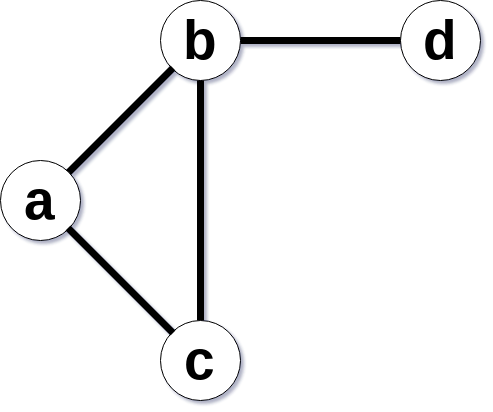
\includegraphics[width=0.25\textwidth]{Images/VertexCover/blank}}
	\only<2>{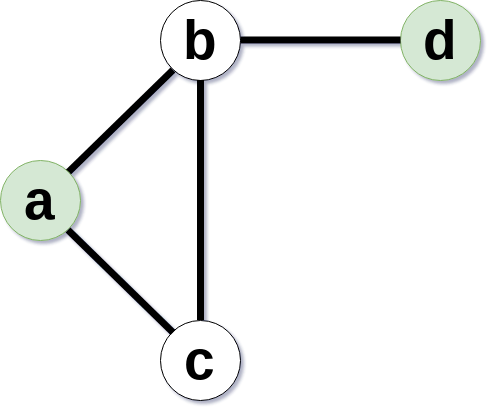
\includegraphics[width=0.25\textwidth]{Images/VertexCover/wrong}}
	\only<3>{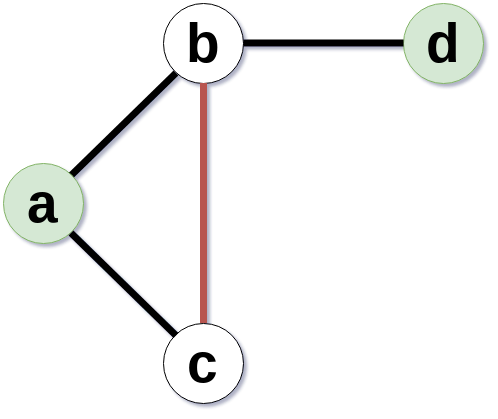
\includegraphics[width=0.25\textwidth]{Images/VertexCover/wrongMarked}}
	\only<4>{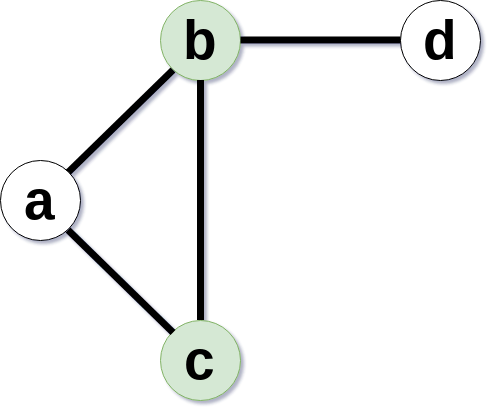
\includegraphics[width=0.25\textwidth]{Images/VertexCover/right}}
	\visible<3>{\alert{(Kein Vertex Cover!)}}
\end{block}
\end{frame}

\newcommand{\ExampleGraphV}{V = \{a,b,c,d\}}
\newcommand{\ExampleGraphE}{E = 
	\begin{Bmatrix}
		\{a,b\},
		\{a,c\},
		\{b,c\},
		\{b,d\}
	\end{Bmatrix}
}

\begin{frame}{\FrameName}
\begin{block}{NP-härte}
	\begin{itemize}[<+->]
			\item Betrachte nur Graphen mit maximalen Knoten-Grad 3
			\item Überführung von Graphen zu Wörtern
			\item Zeige, dass man über die kleinsete Grammatik einen Vertex Cover bestimmen kann
			\item Berechne Upper Bound für effiziente Approximation \linebreak (außer $P=NP$)
		\end{itemize}
\end{block}
\end{frame}

\begin{frame}{\FrameName}
\begin{block}{Beispiel Graph}
	\Gap
	$$\ExampleGraphV$$ 
	$$\ExampleGraphE$$
	\begin{center}
		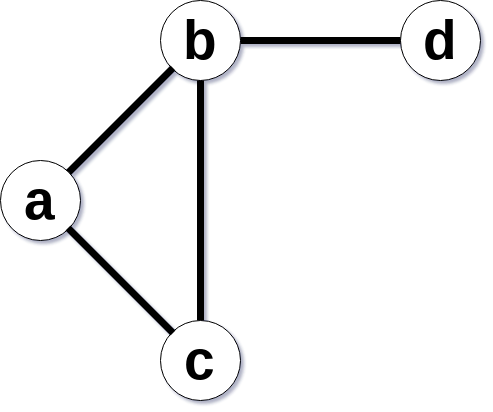
\includegraphics[width=0.35\textwidth]{Images/VertexCover/blank}
	\end{center}
\end{block}
\end{frame}

\newcommand{\ProdRuleOne}[1]{(\# #1 \Fresh #1\#  \Fresh )^2}
\newcommand{\ProdRuleTwo}[1]{\# #1 \#  \Fresh}
\newcommand{\ProdRuleThree}[2]{\# #1 \# #2\#  \Fresh}
\newcommand{\PhantomAlpha}{\phantom{\alpha_{Beispiel} = (}}
\newcommand{\ReductionExample}{
	$
		\alpha_{Beispiel} =
		\textcolor{OrangeRed}{
			\foreach \n in {a,b,c,d}{\ProdRuleOne{\n}}
		} \linebreak
		\PhantomAlpha
		\textcolor{PineGreen}{
			\foreach \n in {a,b,c,d}{\ProdRuleTwo{\n}}
		} \linebreak
		\PhantomAlpha
		\textcolor{RoyalBlue}{
			\ProdRuleThree{a}{b}
			\ProdRuleThree{a}{c}
			\ProdRuleThree{b}{c}
			\ProdRuleThree{b}{d}
		} \linebreak
	$
}

\begin{frame}{\FrameName}
\begin{block}{Graphen zu String überführen}
	\Gap
	$
	\alpha =
	\textcolor{OrangeRed}{
		\prod\limits_{v_i \in V}\ProdRuleOne{v_i}}
	\textcolor{PineGreen}{
		\prod\limits_{v_i \in V}(\ProdRuleTwo{v_i})}
	\textcolor{RoyalBlue}{
			\prod\limits_{\{v_i,v_j\} \in E}(\ProdRuleThree{v_i}{v_j})}
	$

	
	\visible<2>{
		\Gap
			$\ExampleGraphV; \ExampleGraphE$ \newline
		\Gap
		\ReductionExample
	}
\end{block}
\end{frame}

\begin{frame}{\FrameName}
	\ReductionExample
\begin{block}{Eigenschaften der kleinsten Grammatik}
	\begin{itemize}[<+->]
		\item Jedes Nichtterminal expandiert zu $\#v_i$, $v_i\#$ oder $\#v_i\#$
		\item Enthält Regeln der Form $T_j \rightarrow \#v_i$ und $T_j \rightarrow v_i\#$
		\item $C = \{v_i \in V | \exists T_j \rightarrow \#v_i\#\}$ ist (minimale) Vertex Cover
	\end{itemize}
\end{block}
\end{frame}

\begin{frame}{\FrameName}
\begin{block}{Approximation Ratio}
	\begin{itemize}[<+->]
		\item $m^* = 15|V| + 3|E| + |C|$
		\item Es ist ($NP$) hart Vertex Cover kleiner als $\frac{145}{144} \cdot |C|$ zu finden ($\frac{145}{144}\approx 1,006944...$)
		\item $\rho = \frac{15|V| + 3|E| + \frac{145}{144}|C|}{15|V| + 3|E| + |C|}$
		\item $\rho \geq \frac{15|V| + 3 \cdot \frac{3}{2}|V| + \frac{145}{144}(\frac{1}{3}|V|)}{15|V| + 3 \cdot \frac{3}{2}|V| + \frac{1}{3}|V|} = \frac{8569}{8568} \approx 1,0001167...$
	\end{itemize}
\end{block}
\end{frame}

\section{Approximationsalgorithmen}

\begin{frame}{\FrameName}
	\begin{itemize}[<+->]
		\item LZ78
		\item Bisection 
		\item Sequential
		\item Global algorithms
		% \setlength{\itemindent}{1cm}
		\begin{itemize}
			\item[-] Longest Match
			\item[-] Greedy
			\item[-] Re-Pair
		\end{itemize}
	\end{itemize}
\end{frame}

\subsection{Vorüberlegungen}

\newcommand{\LowerBound}{\textcolor{TealBlue}{f_l(n)}}
\newcommand{\UpperBound}{\textcolor{Salmon}{f_u(n)}}



\subsection{LZ78}

\begin{frame}{\FrameName}
\begin{block}{LZ78 - Datenstrukturen}
	\begin{itemize}[<+->]
		\item Strings werden als Sequenzen von Paaren $(i,c)$ dargestellt \linebreak \Hint{$i$...Index eines Vorgänger-Paares oder $0$$; c \in \Sigma$}
		\item Jedes Paar repräsentiert einen Substring
		\item Wenn $i$ gleich $0$ dann ist dieser Substring gleich $c$
		\item Andernfalls ist der Substring des $i$-ten Parres gefolgt von $c$
	\end{itemize}
\end{block}
\end{frame}

\begin{frame}{\FrameName}
\begin{block}{Beispiel}
	\Gap
	\Gap
	\only<1>{
		
\includegraphics[width=\textwidth]{Images/LZ78/blank}}
	\only<2>{
		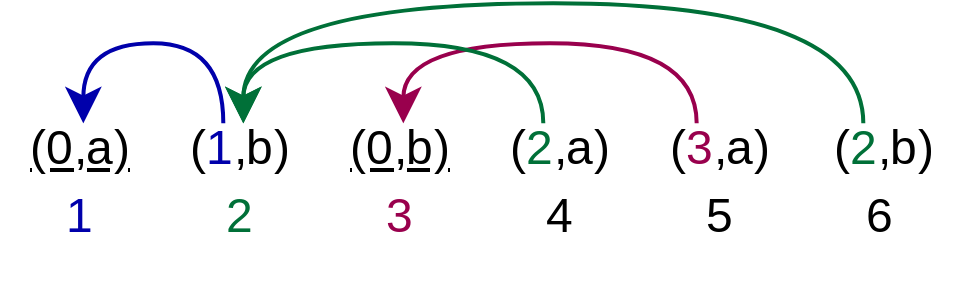
\includegraphics[width=\textwidth]{Images/LZ78/withRef}}
	\only<3>{
		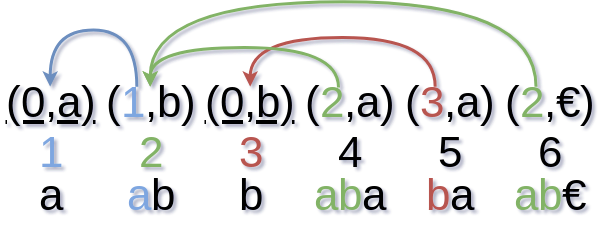
\includegraphics[width=\textwidth]{Images/LZ78/full}}
\end{block}
\end{frame}

\begin{frame}{\FrameName}
\begin{block}{LZ78 - Algorithmus}
	\begin{itemize}[<+->]
		\item String wird Schrittweise in einem Durchlauf von links nach rechts in eine Sequenz von Paaren übersetzt
		\item Finde in jedem Schritt das kürzeste Präfix $\gamma$ des verbleibenden Strings das nicht Expansion eines bereits erzeugten Paars ist
		\item Am Ende des Strings muss eventuell ein weiteres Zeichen hinzugefügt werden
		\item Ein neues Paar wird an die Liste angehangen:
		\begin{enumerate}
			\item<4-> Wenn da $\gamma = 1$ ist füge $(0,\gamma)$ hinzu
			\item<5-> Andernfalls ist $\gamma = \alpha c$. \linebreak $\alpha$ ... Expansion eines Paars mit dem Index $i_\alpha$ \linebreak $\Rightarrow$ Paar: $(i,c)$
		\end{enumerate}
	\end{itemize}
\end{block}
\end{frame}

% Marking string sequence
\newcommand{\M}[1]{\textcolor{OrangeRed}{#1}}

\begin{frame}{\FrameName}
\begin{block}{Beispiel}
	\begin{description}[<+->]
		\item \M{a}abbababaab\euro
		\item (0,a) \M{ab}bababaab\euro
		\item (0,a) (1,b) \M{b}ababaab\euro
		\item (0,a) (1,b) (0,b) \M{aba}baab\euro
		\item (0,a) (1,b) (0,b) (2,a) \M{ba}ab\euro
		\item (0,a) (1,b) (0,b) (2,a) (3,a) \M{ab\euro}
		\item (0,a) (1,b) (0,b) (2,a) (3,a) (2,\euro)
	\end{description}
\end{block}
\end{frame}

\begin{frame}{\FrameName}
\begin{block}{LowerBound}
	\begin{center}
		\fbox{$ \alpha_k = a^{k(k+1)/2}(ba^k)^{(k+1)^2} $}
	\end{center}
	\begin{itemize}[<+->]
		\item $|\alpha_k | = k \frac{k+1}{2} + (1+k)(k+1)^2$ \linebreak
			$\phantom{|\alpha_k |} = k^3 + \frac{7}{2}k^2 + \frac{7}{2}k + 1$
		\item $ n = |\alpha_k | \in \Theta(k^3)$
	\end{itemize}
\end{block}
\end{frame}

\begin{frame}{\FrameName}
\begin{block}{UpperBound $m^*$}
	\begin{center}
		\fbox{$ \alpha_k = a^{k(k+1)/2}(ba^k)^{(k+1)^2} $}
	\end{center}
	\begin{itemize}[<+->]
		\item $m^* \in \mathcal{O}(1+ log(\frac{k^2+k}{2}) + log(k+1)^2 + 1+ log(k))$
		\item $m^* \in \mathcal{O}(log \thinspace k)$
		\item $m^* \in \mathcal{O}(log \thinspace n^\frac{1}{3}) = \mathcal{O}(log \thinspace n)$
	\end{itemize}
\end{block}
\end{frame}

\begin{frame}{\FrameName}
\begin{block}{LowerBound m}
	\begin{center}
		\fbox{$ \alpha_k = a^{k(k+1)/2}(ba^k)^{(k+1)^2} $}
	\end{center}
	\begin{itemize}[<+->]
		\item String wird in zwei Phasen in eine Paar-Sequenz übersetzt
		\item Erste Phase: alle Strings $a...a^k$ zu Paaren übersetzt
		\item Zweite Phase: $a^iba^j$ für alle $i,j \in [0,k]$ wird ein Paar erstellt
		\item $m \in \Omega(\sum_{z=1}^k z + (k+1)^2) = \Omega(k^2)$
		\item $m \in \Omega(n^{2/3})$
	\end{itemize}
\end{block}
\end{frame}

\begin{frame}{\FrameName}
\begin{block}{LowerBound}
	\begin{center}
		\fbox{$ \alpha_k = a^{k(k+1)/2}(ba^k)^{(k+1)^2} $}
	\end{center}
	\begin{itemize}[<+->]
		\item $m^* \in \mathcal{O}(log \thinspace n)$
		\item $m \in \Omega(n^{2/3})$
		\item $a(n) \in \Omega(\frac{n^{2/3}}{log \thinspace n})$
	\end{itemize}
\end{block}
\end{frame}


\subsection{Global Algorithms}
\begin{frame}{\FrameName}
	\begin{block}{Global Algorithms}
    \begin{itemize}[<+->]
      \item Klasse von Algorithmen
      \item Haben alle ein upper bound von $\mathcal{O}((\frac{n}{log(n)})^{\frac{2}{3}})$
      \item Lower bounds sind sehr schlecht
    \end{itemize}
\end{block}
\end{frame}

\begin{frame}{\FrameName}
	\begin{block}{Global Algorithms - Verfahren}
    \begin{itemize}[<+->]
      \item Grammatik schrittweise verbessert
      \item Initialisiere Grammatik mit $S \rightarrow \alpha$
      \item Wähle einen String $\gamma$
      \item Füge $T \rightarrow \gamma$ \Hint{(T... neues Nichtterminal)}
      \item Traversiere alle anderen Regeln von links nach rechts und ersetze vorkommen von $\gamma$ durch $T$
    \end{itemize}
\end{block}
\end{frame}

\begin{frame}{\FrameName}
	\begin{block}{Auswahl von $\gamma$}
    \begin{itemize}[<+->]
      \item $|\gamma| \ge 2$
      \item $\gamma$ kommst mind. zwei mal in Grammatik vor \linebreak \Hint{(ohne Überschneidung)}
      \item Alle Strings länger als $\gamma$ kommen seltener vor
    \end{itemize}
\end{block}
\end{frame}

\begin{frame}{\FrameName}
	\begin{block}{Upper Bound}
    \begin{itemize}[<+->]
      \item Ähnlich upper bound von LZ78
      \item Auflistung von Substrings der Länge 2
      \item Einordnung in Gruppen
      \item Abschätzen der Gesamt-Expansionslänge der Gruppen
    \end{itemize}
\end{block}
\end{frame}

\begin{frame}{\FrameName}
	\begin{block}{Upper Bound (1/4)}
    \begin{itemize}[<+->]
      \item Wähle $\frac{2}{9}m$ Substrings der Länge 2 \linebreak \Hint{(ohne Überschneidung)}
      \item ist immer möglich
    \end{itemize}
\end{block}
\end{frame}

\begin{frame}{\FrameName}
	\begin{block}{Upper Bound (2/4)}
    \begin{itemize}[<+->]
      \item Sortiere Substrings aufsteigend nach deren Expansionslänge
      \item Füge die ersten $2m^*$ Substrings der ersten Gruppe hinzu
      \item Füge die nächsten $3m^*$ Substrings der zweiten Gruppe hinzu
      \item usw. ...(bis zur Gruppe mit $gm^*$ Elementen)
      \item $2m^* + 3m^* + ... + gm^* (g+1)m^* > \frac{2}{9}m$
      \item $m^*\sum_{k=2}^{g+1}k = m^* (\frac{g^2}{2} + \frac{3g}{2}) > \frac{2}{9}m$
      \item $m\in \mathcal{O}(g^2 m^*)$
    \end{itemize}
\end{block}
\end{frame}

\begin{frame}{\FrameName}
	\begin{block}{Upper Bound (3/4)}
    \begin{itemize}[<+->]
      \item Sei $\sigma = $ "Gesamt-Expansionslänge"
      \item Für jedes $\alpha$ in i-ten Gruppen gilt: $|\langle \alpha \rangle | \ge i+1$ \Hint{(mk-Lemma)}
      \item $2^2m^* + 3^2m^* + ... + g^2m^* \le \sigma$
      \item $\sigma \le 2n$
      \item $2^2m^* + 3^2m^* + ... + g^2m^* \le 2n$
      \item $m^* \sum_{k=2}^{g}k^2 = m^* (\frac{g^3}{3} + \frac{g^2}{2} + \frac{g}{6} - 1) \le 2n$
      \item $g^3 \in \mathcal{O}(\frac{n}{m^*}) \Rightarrow g \in \mathcal{O}((\frac{n}{m^*})^{\frac{1}{3}})$
    \end{itemize}
\end{block}
\end{frame}

\begin{frame}{\FrameName}
	\begin{block}{Upper Bound (4/4)}
    \begin{itemize}[<+->]
      \item $m\in \mathcal{O}(g^2 m^*)$ und $g \in \mathcal{O}((\frac{n}{m^*})^{\frac{1}{3}})$
      \item $m \in \mathcal{O}((\frac{n}{m^*})^{\frac{2}{3}} m^*) = \mathcal{O}((\frac{n}{log (n)})^{\frac{2}{3}} m^*)$
      \item $a(n) = \max\limits_{\alpha \in \Sigma^n} \frac{m}{m^*} \in \mathcal{O}((\frac{n}{log(n)})^{\frac{2}{3}}) \qed$
    \end{itemize}
\end{block}
\end{frame}

\begin{frame}{\FrameName}
	\begin{block}{Greedy}
    \Gap
    In jeder Iteration wird das $\gamma $ gewählt welches die Größe der Grammatik am meisten senkt.
\end{block}
\end{frame}

\begin{frame}{\FrameName}
	\begin{block}{Lower bound}
    \Gap
    
\end{block}
\end{frame}


\section{Zusammenfassung}
\subsection{}


\begin{frame}{\FrameName}
    \begin{itemize}[<+->]
      \item interessant für Kompression und Musterkennung (NLP)
      \item Optimale Lösen ist NP-hart
      \item Mit bekannten Verfahren lassen sich Approximation generieren (zB LZ78)
      \item Global algorithms relativ unerforscht
    \end{itemize}

  \end{frame}

\end{document}
